\section{Ansätze zur Entity-Resolution}

\subsection{Trivialer Ansatz}
\begin{frame}
	\vspace*{-0.15cm}
	\hspace*{-.35cm} \textbf{\underline{Transformation:}}
	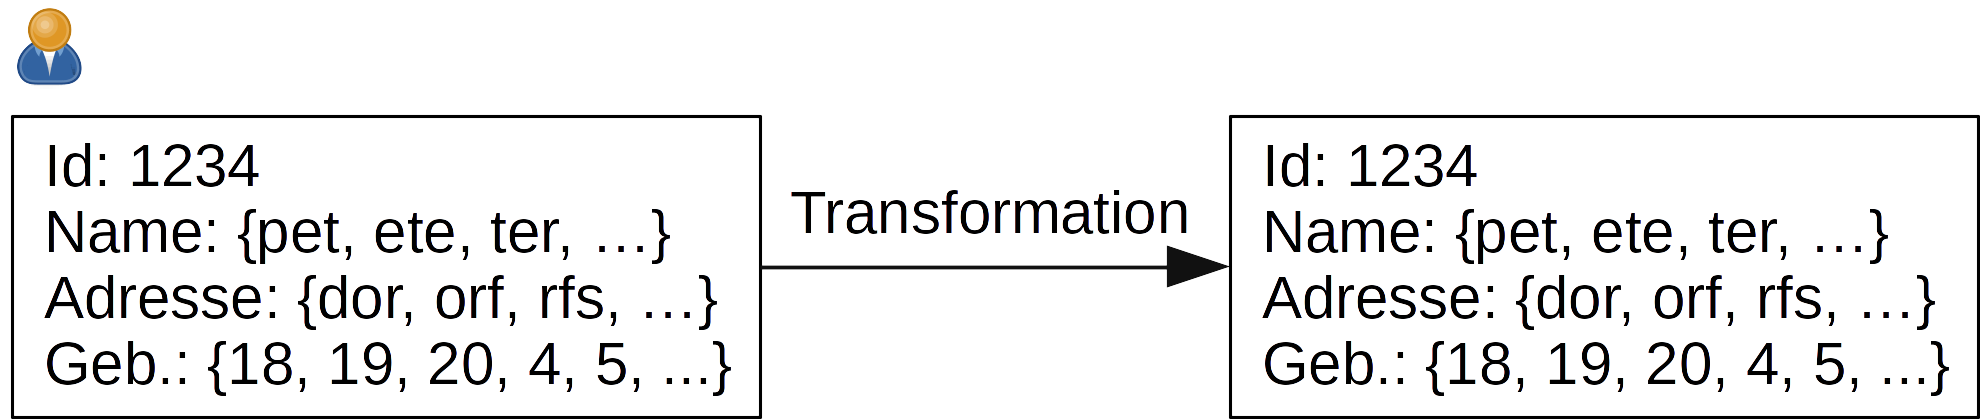
\includegraphics[width=1.01\textwidth]{Bilder/Transformation_Strings.png}
	\vspace*{0.35cm}

	\hspace*{-.35cm} \textbf{\underline{Ähnlichkeitsfunktion:}}
	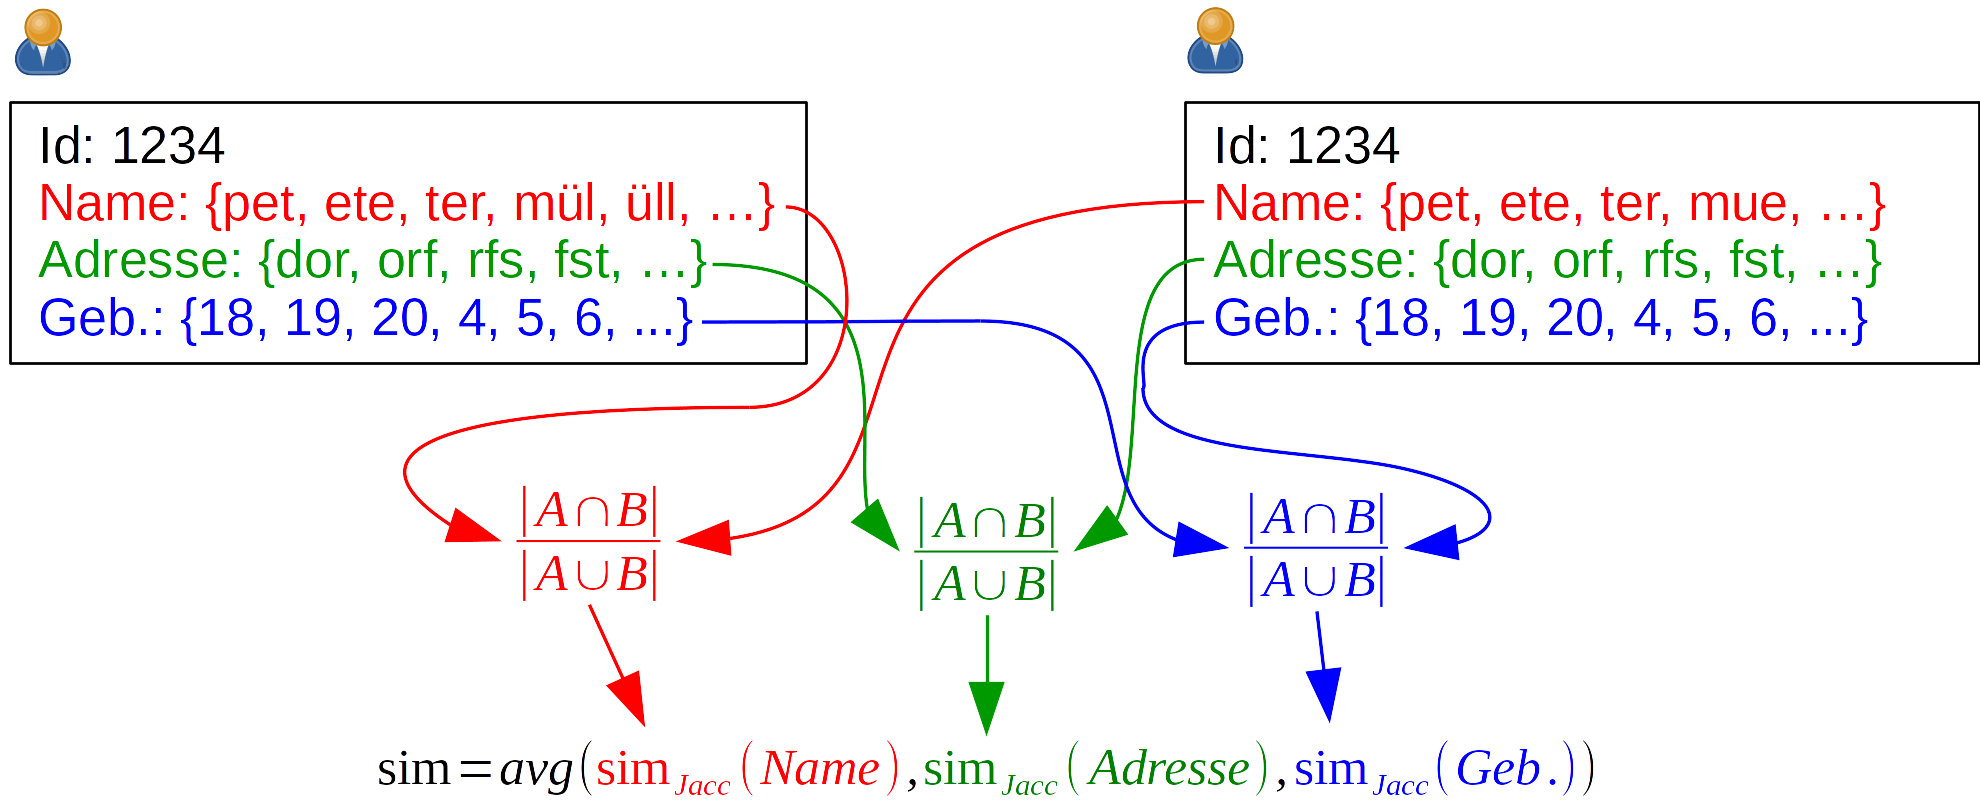
\includegraphics[width=1.01\textwidth]{Bilder/sim_strings.png}
\end{frame}

\subsection{Sortier-Ansatz}
\begin{frame}
	\begin{itemize}
		\setlength\itemsep{\stdItemSep}
		\item Analog zu Sort-Merge-Verbund\footnotemark
		\begin{itemize}
			\setlength\itemsep{\stdItemSep}
			\vspace*{\stdItemSep}
			\item Während Import: Sortiere Mengen
			\item Während ER: Berechne Kardinalität der Schnittmenge in $\mathcal{O}(n)$
			\begin{itemize}
				\setlength\itemsep{\stdItemSep}
				\vspace*{\stdItemSep}
				\item Schritthaltende Traversierung der sortierten Mengen
			\end{itemize}
		\end{itemize}
	\end{itemize}

	\footnotetext[1]{Siehe Vorlesung Implementierung von Datenbanksystemen}
\end{frame}

\subsection{Bit-Array-Ansatz}
\begin{frame}
	\frametitle{Einschub: Bloom-Filter}

	\uncover<1-1>
	{
		\begin{tikzpicture}[overlay]
			\node (start) at (6.1, -0.47) {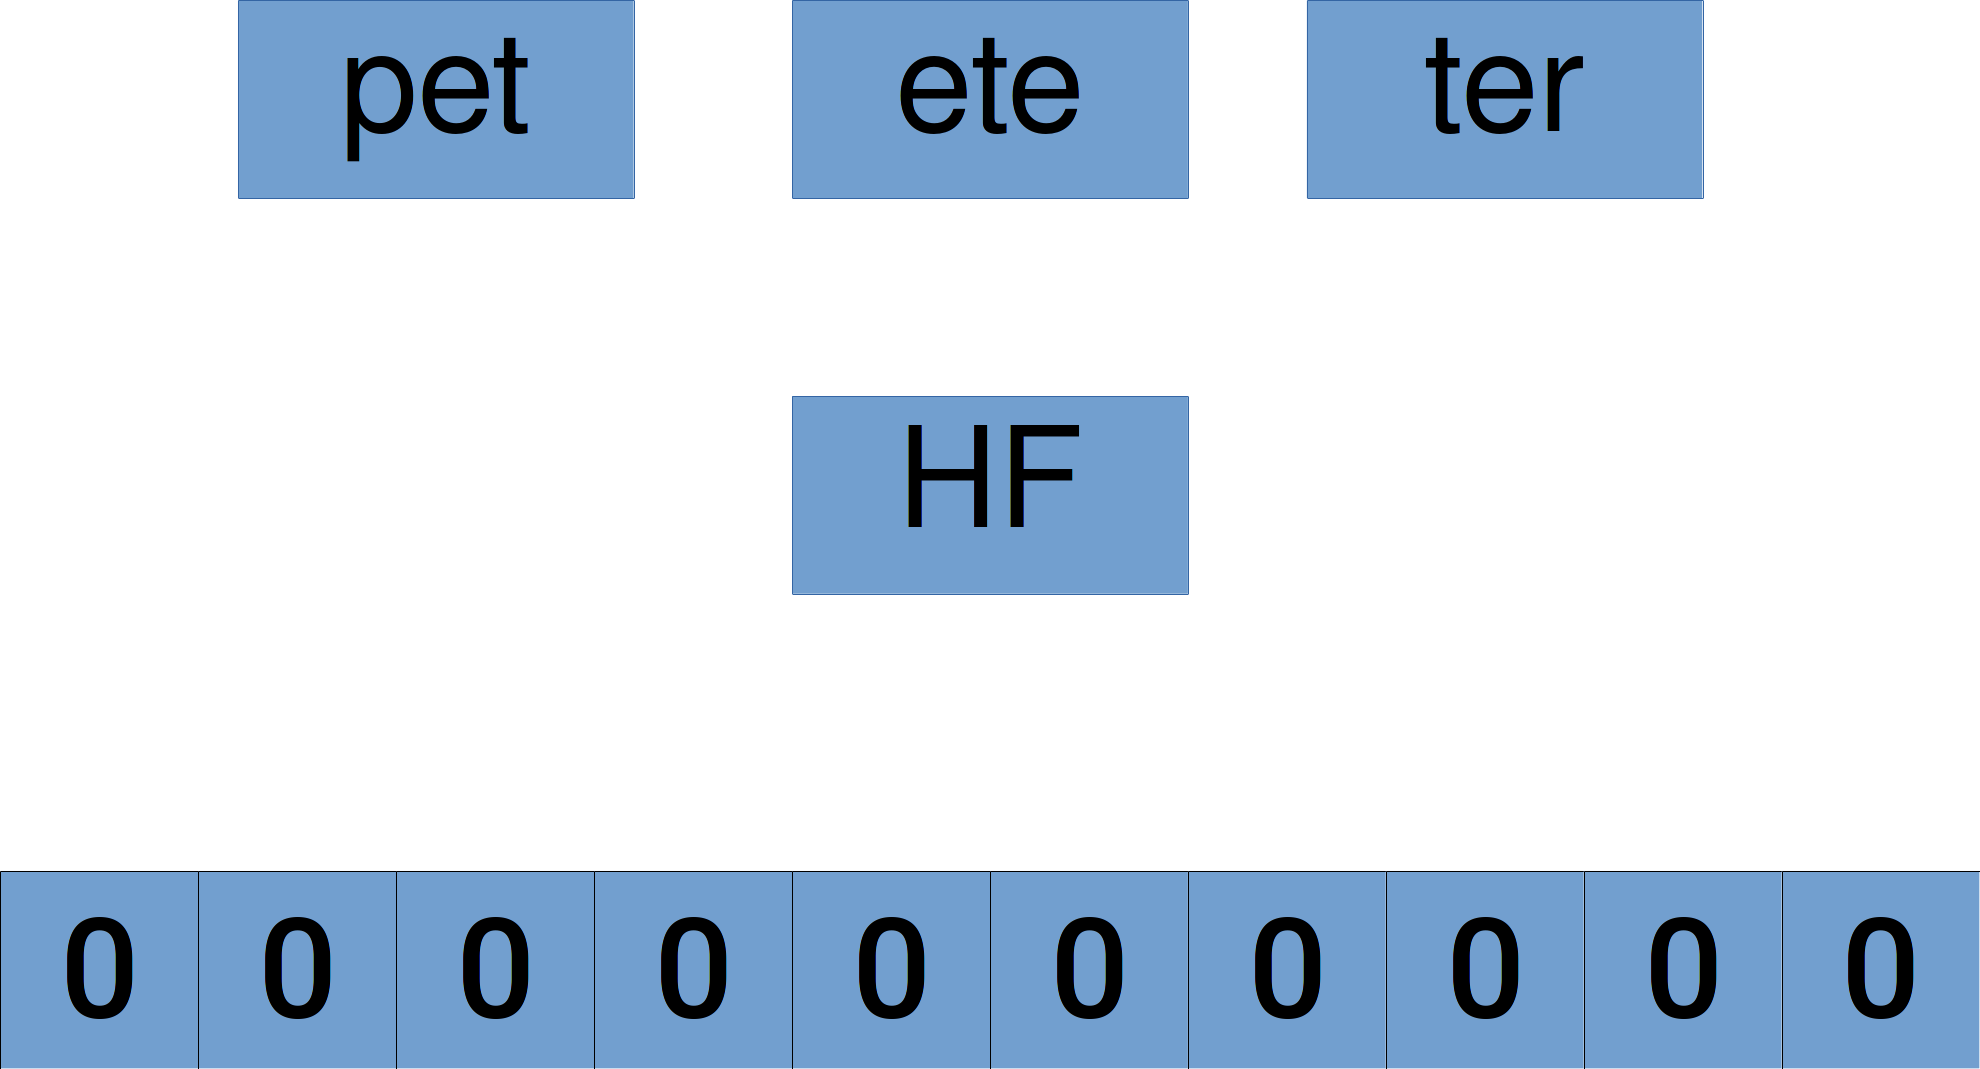
\includegraphics[width=0.9\textwidth]{Bilder/bloomfilter_example_insert_01.png}};
		\end{tikzpicture}
	}

	\uncover<2-2>
	{
		\begin{tikzpicture}[overlay]
			\node (start) at (6.1, 0) {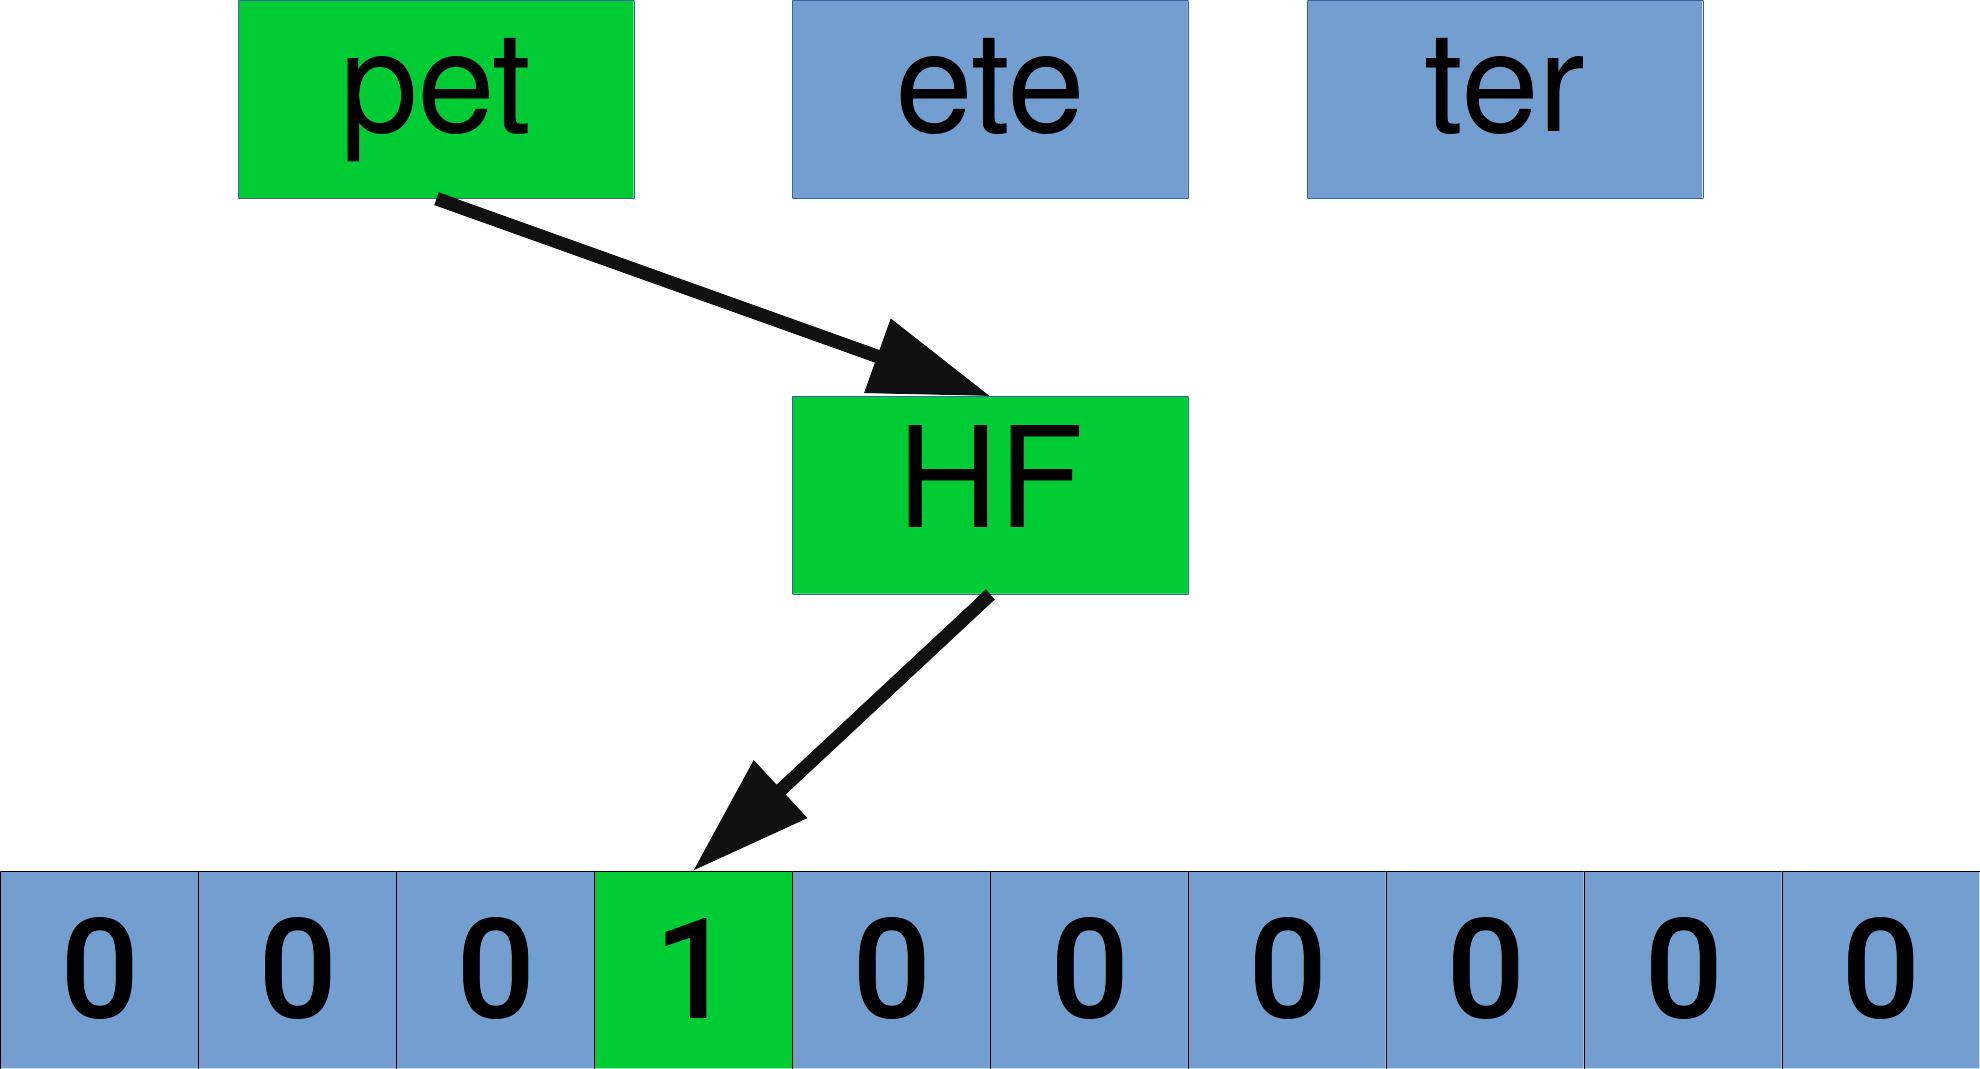
\includegraphics[width=0.9\textwidth]{Bilder/bloomfilter_example_insert_02.png}};
		\end{tikzpicture}
	}

	\uncover<3-3>
	{
		\begin{tikzpicture}[overlay]
			\node (start) at (6.1, 0.47) {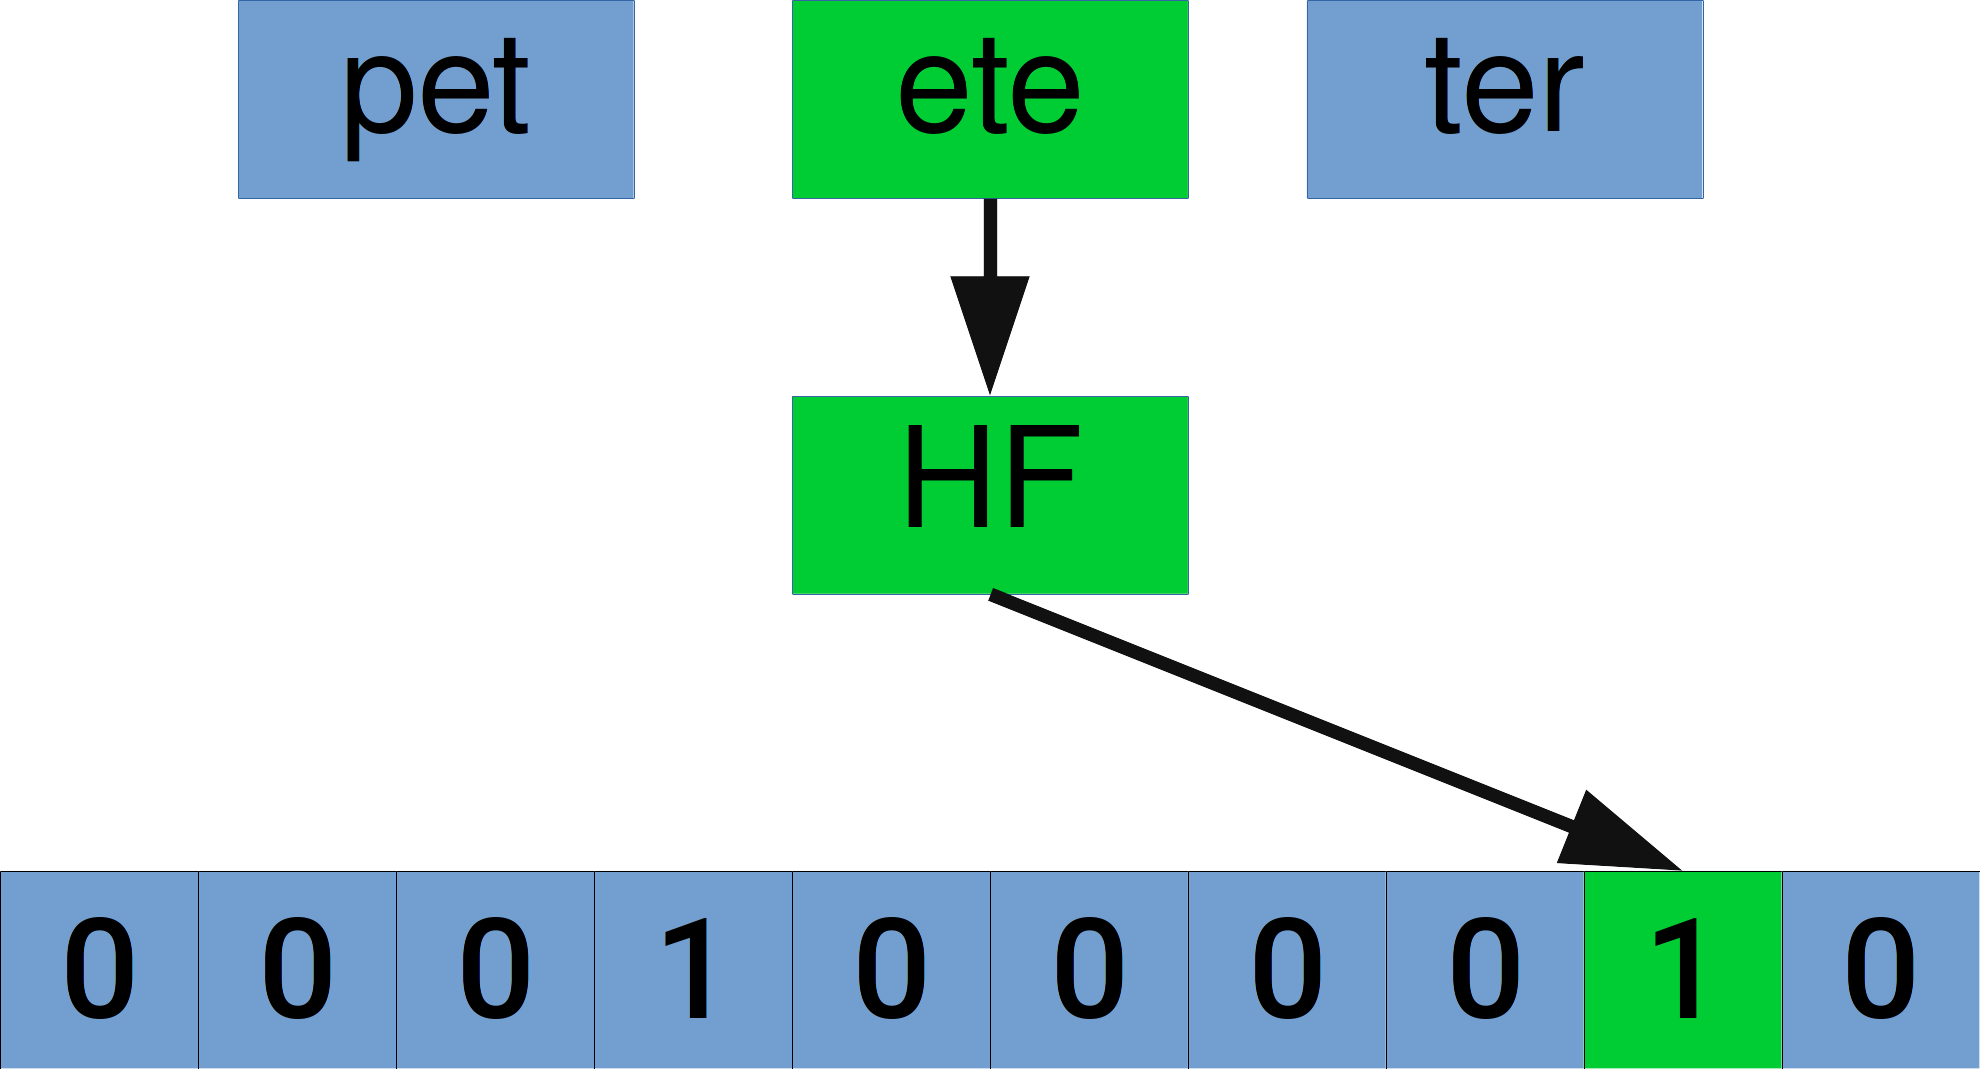
\includegraphics[width=0.9\textwidth]{Bilder/bloomfilter_example_insert_03.png}};
		\end{tikzpicture}
	}

	\uncover<4-4>
	{
		\begin{tikzpicture}[overlay]
			\node (start) at (6.1, 0.94) {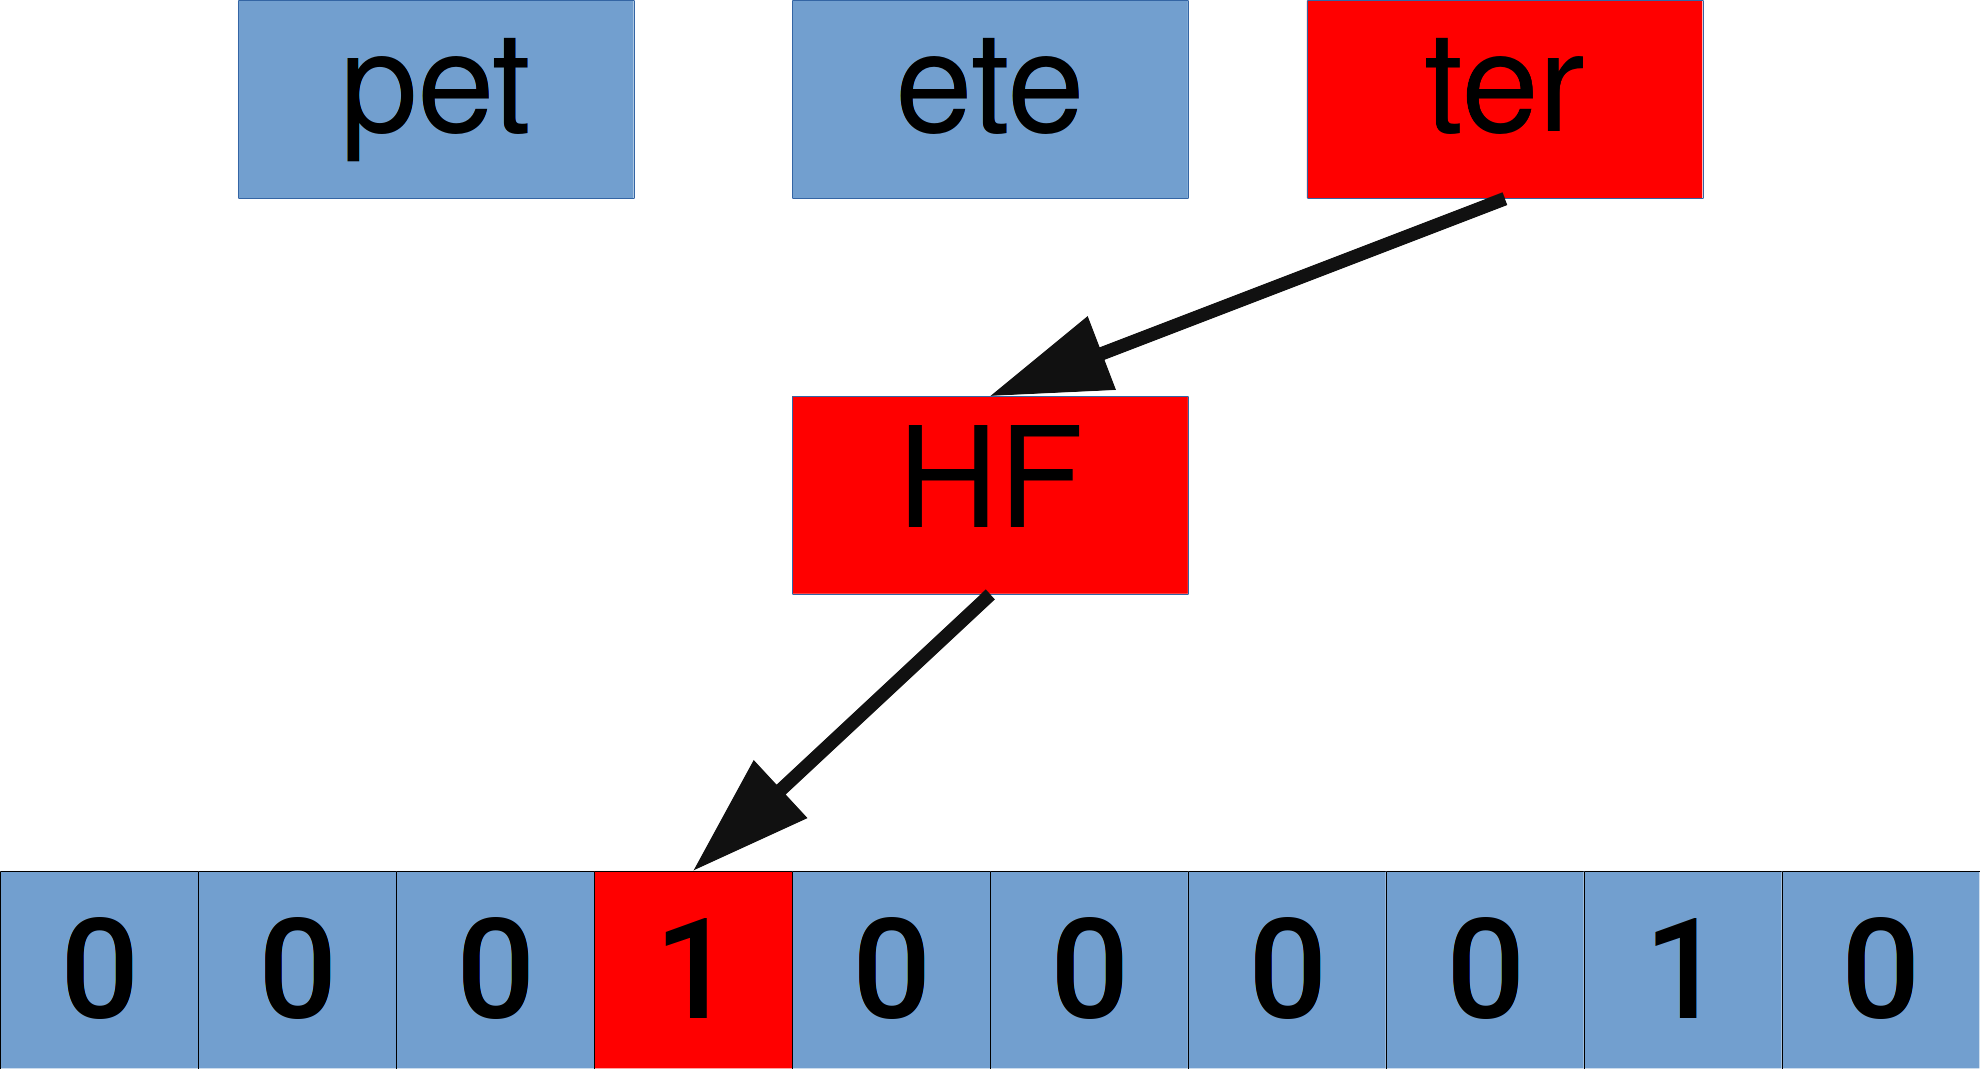
\includegraphics[width=0.9\textwidth]{Bilder/bloomfilter_example_insert_04.png}};
		\end{tikzpicture}
	}

	\begin{tikzpicture}[overlay]
		\node at (11.5, 1.5)
		{
			\begin{footnotesize}
			\begin{varwidth}{0.4\textwidth}
			\textbf{Hier:}
			\begin{itemize}
				\item Immer genau eine Hashfunktion!
			\end{itemize}
			\end{varwidth}
			\end{footnotesize}
		};
	\end{tikzpicture}
\end{frame}

\begin{frame}
	\vspace*{-0.1cm}
	\hspace*{-.35cm} \textbf{\underline{Transformation:}}
	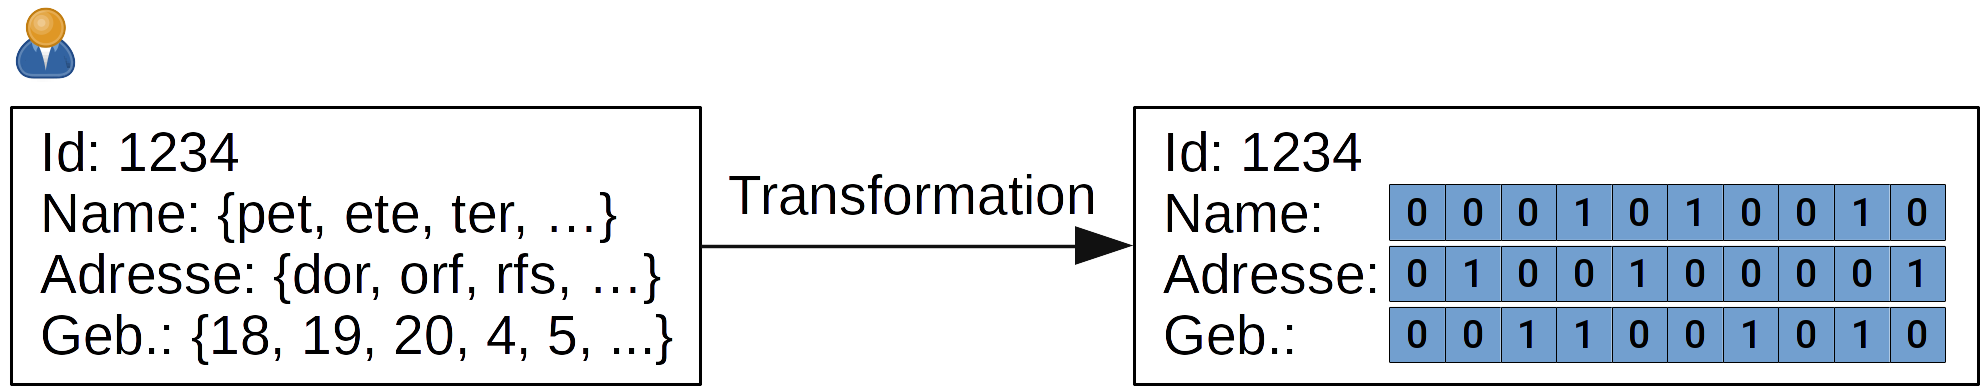
\includegraphics[width=1.01\textwidth]{Bilder/Transformation_Bitarray.png}
	\vspace*{0.5cm}

	\hspace*{-.35cm} \textbf{\underline{Ähnlichkeitsfunktion:}}
	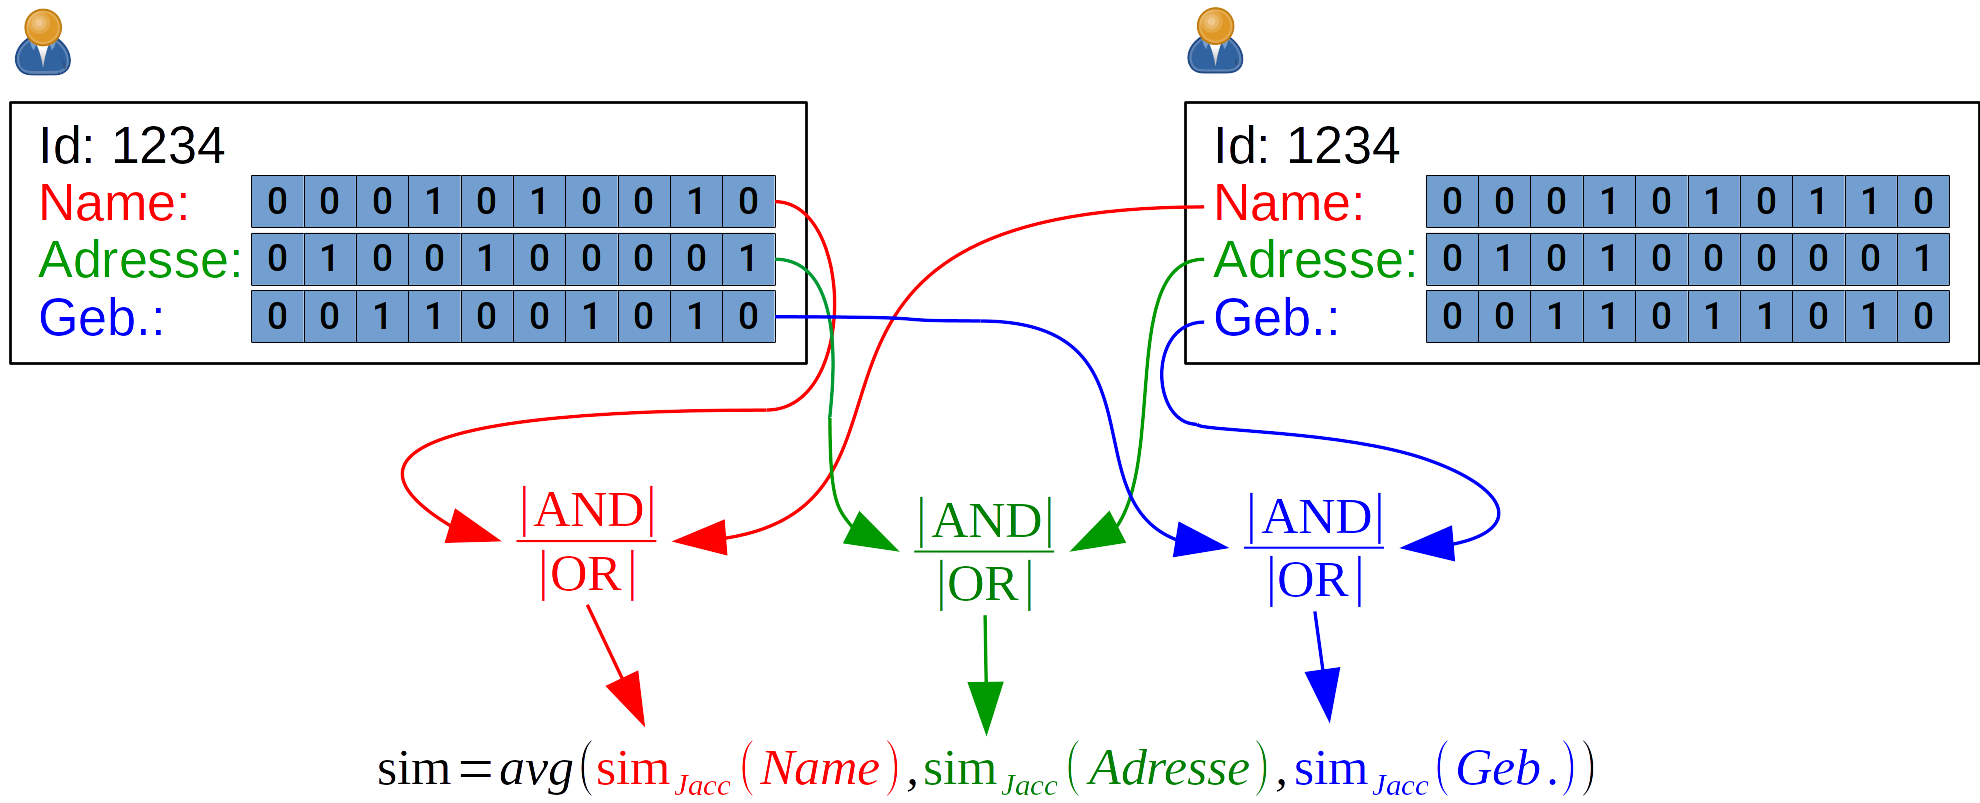
\includegraphics[width=1.01\textwidth]{Bilder/sim_bitarray.png}
\end{frame}

\subsection{Vergleich}
\begin{frame}
	\vspace*{-.025cm}
	\hspace*{-.5cm}
	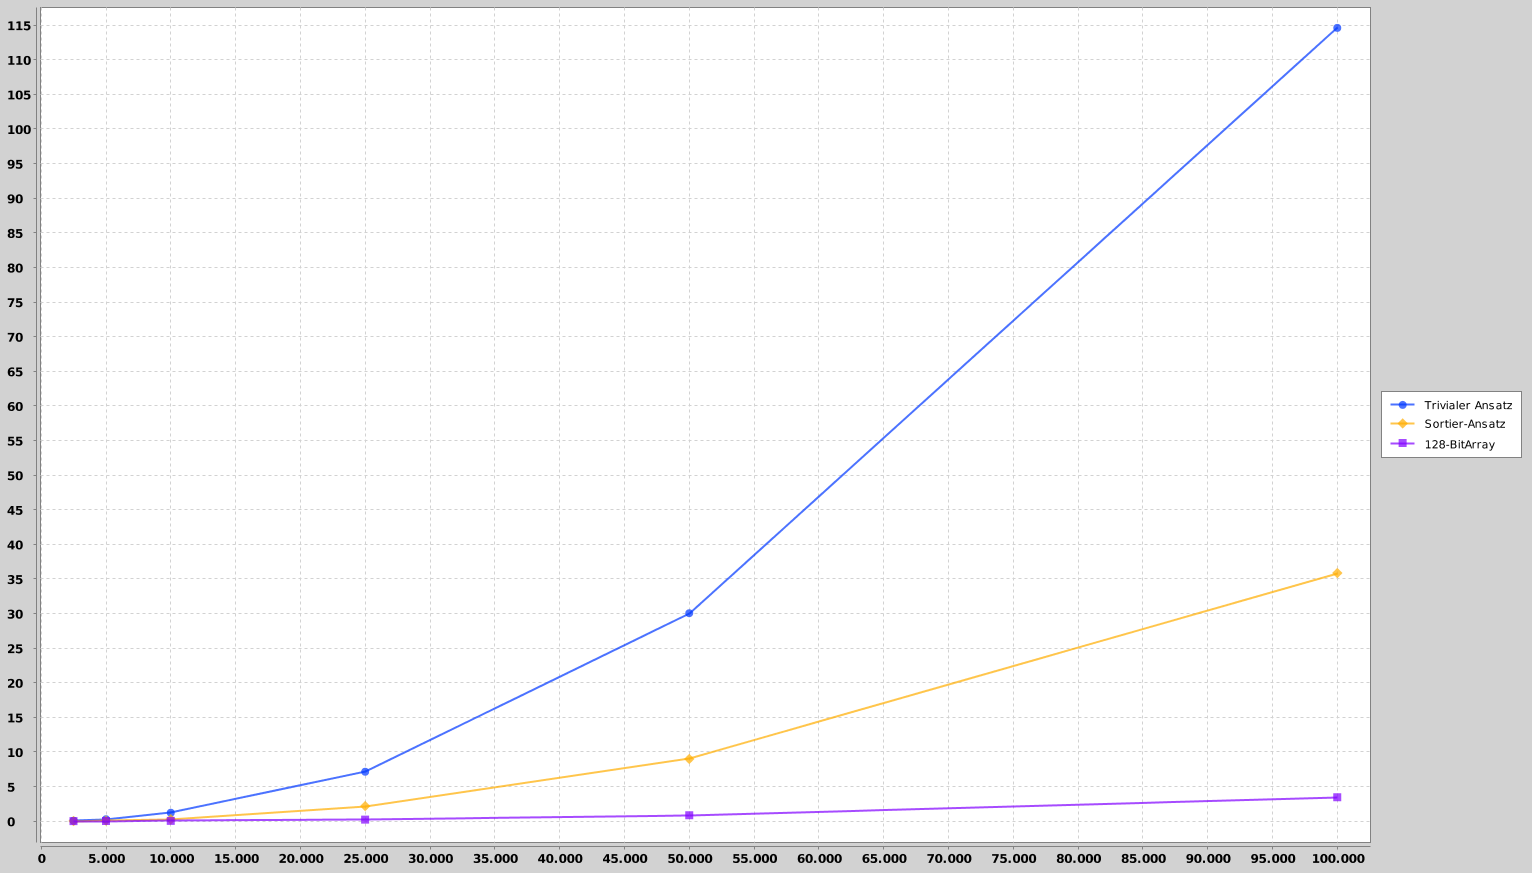
\includegraphics[width=1.07\textwidth, height=1.02\textheight]{Bilder/evaluation_runtime_for_threshold_0_7_trigram_one_fuzzy_date.png}

	\begin{tikzpicture}[overlay]
		\node at (4.7, 7)
		{
			\begin{footnotesize}
			\begin{varwidth}{0.75\textwidth}
			\textbf{Ausführungszeit in Minuten}
			\begin{itemize}
				\item für unterschiedlich große Datensätze
				\item Parameter
				\begin{itemize}
					\item Trigramme
					\item Threshold: $0.7$
					\item Datumsunschärfe: $1$
				\end{itemize}
				\item Testsystem
				\begin{itemize}
					\item CPU: 8 Kerne (HT) @ 3.4 GHz
					\item RAM: 16 GB
				\end{itemize}
			\end{itemize}
			\end{varwidth}
			\end{footnotesize}
		};
	\end{tikzpicture}

\end{frame}

\begin{frame}
	\vspace*{-.025cm}
	\hspace*{-.5cm}
	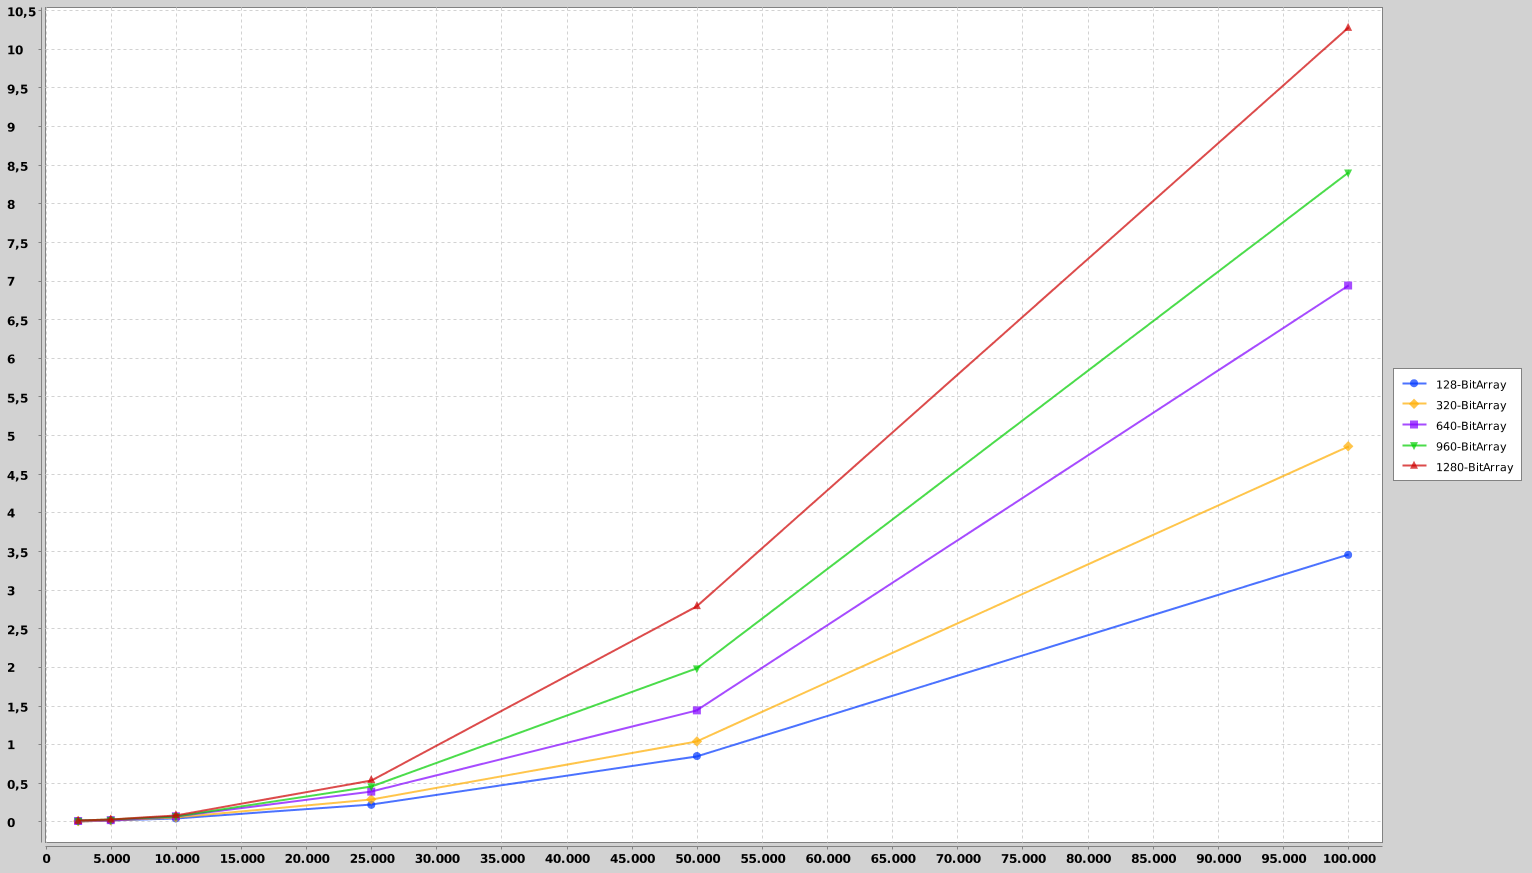
\includegraphics[width=1.07\textwidth, height=1.02\textheight]{Bilder/evaluation_runtime_bit_array_size_for_threshold_0_7_trigram_one_fuzzy_date.png}

	\begin{tikzpicture}[overlay]
		\node at (4.7, 7)
		{
			\begin{footnotesize}
			\begin{varwidth}{0.75\textwidth}
			\textbf{Ausführungszeit verschiedener Bit-Array-Größen in Minuten}
			\begin{itemize}
				\item für unterschiedlich große Datensätze
				\item Parameter
				\begin{itemize}
					\item Trigramme
					\item Threshold: $0.7$
					\item Datumsunschärfe: $1$
				\end{itemize}
				\item Testsystem
				\begin{itemize}
					\item CPU: 8 Kerne (HT) @ 3.4 GHz
					\item RAM: 16 GB
				\end{itemize}
			\end{itemize}
			\end{varwidth}
			\end{footnotesize}
		};
	\end{tikzpicture}

\end{frame}

\begin{frame}
	\hspace*{-.35cm} \textbf{\underline{Absolute Werte:}}
	\hspace*{-.5cm}
	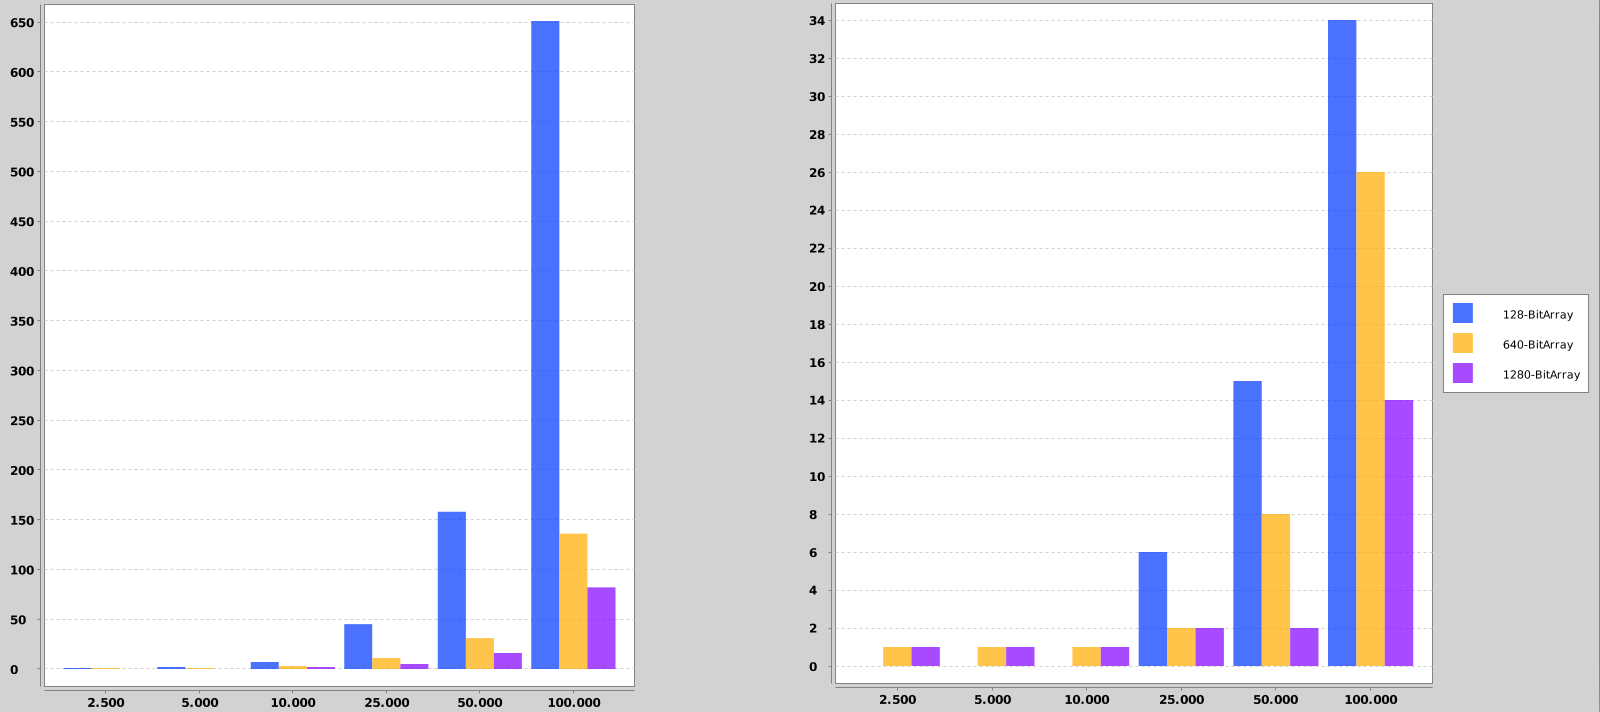
\includegraphics[width=1.07\textwidth, height=0.8\textheight]{Bilder/false_negative_false_positive_threshold_0_7_trigram_one_fuzzy_date.png}
	\begin{tikzpicture}[overlay]
		\node at (-10., 6)
		{
			\begin{footnotesize}
			\begin{varwidth}{0.4\textwidth}
			\textbf{False Positives}
			\begin{itemize}
				\item Trigramme
				\item Threshold: $0.7$
				\item Datumsunschärfe: $1$
			\end{itemize}
			\end{varwidth}
			\end{footnotesize}
		};

		\node at (-3.6, 6)
		{
			\begin{footnotesize}
			\begin{varwidth}{0.4\textwidth}
			\textbf{False Negatives}
			\begin{itemize}
				\item Trigramme
				\item Threshold: $0.7$
				\item Datumsunschärfe: $1$
			\end{itemize}
			\end{varwidth}
			\end{footnotesize}
		};

		\node (one) at (-12.2, 1) {\tiny $1$};
		\node (zero) at (-11.8, 1) {\tiny $0$};


		\node (a) at (-12.3, 0.32) {};
		\node (b) at (-12, 0.32) {};
		\node (c) at (-11.8, 0.32) {};

		\path [draw, ->] (one) -- (a);	
		\path [draw, ->] (one) -- (b);
		\path [draw, ->] (zero) -- (c);
	\end{tikzpicture}

	\uncover<2->
	{
		\begin{center}
		\begin{scriptsize}
		\begin{tabular}{l|c|c|c}
			& 128-Bit & 640-Bit & 1280-Bit\\
			\hline
			Precision & 0.955 & 0.990 & 0.994 \\
			\hline
			Recall & 0.998 & 0.998 & 0.999 \\
		\end{tabular}
		\end{scriptsize}
		\end{center}
		\begin{tikzpicture}[overlay]
			\node (a) at (10.7, 1.6) {};
			\node (b) at (9, 1) {};
			\node (c) at (4, 1.6) {};
			\node (d) at (4.7, 1) {};

			\path [draw, ->, green, very thick] (a) -- (b);	
			\path [draw, ->, green, very thick] (c) -- (d);	
		\end{tikzpicture}
	}
\end{frame}
